\documentclass{standalone}
\usepackage{pgfplots}
\usepackage{lmodern}
\pgfplotsset{compat=1.17}

\begin{document}
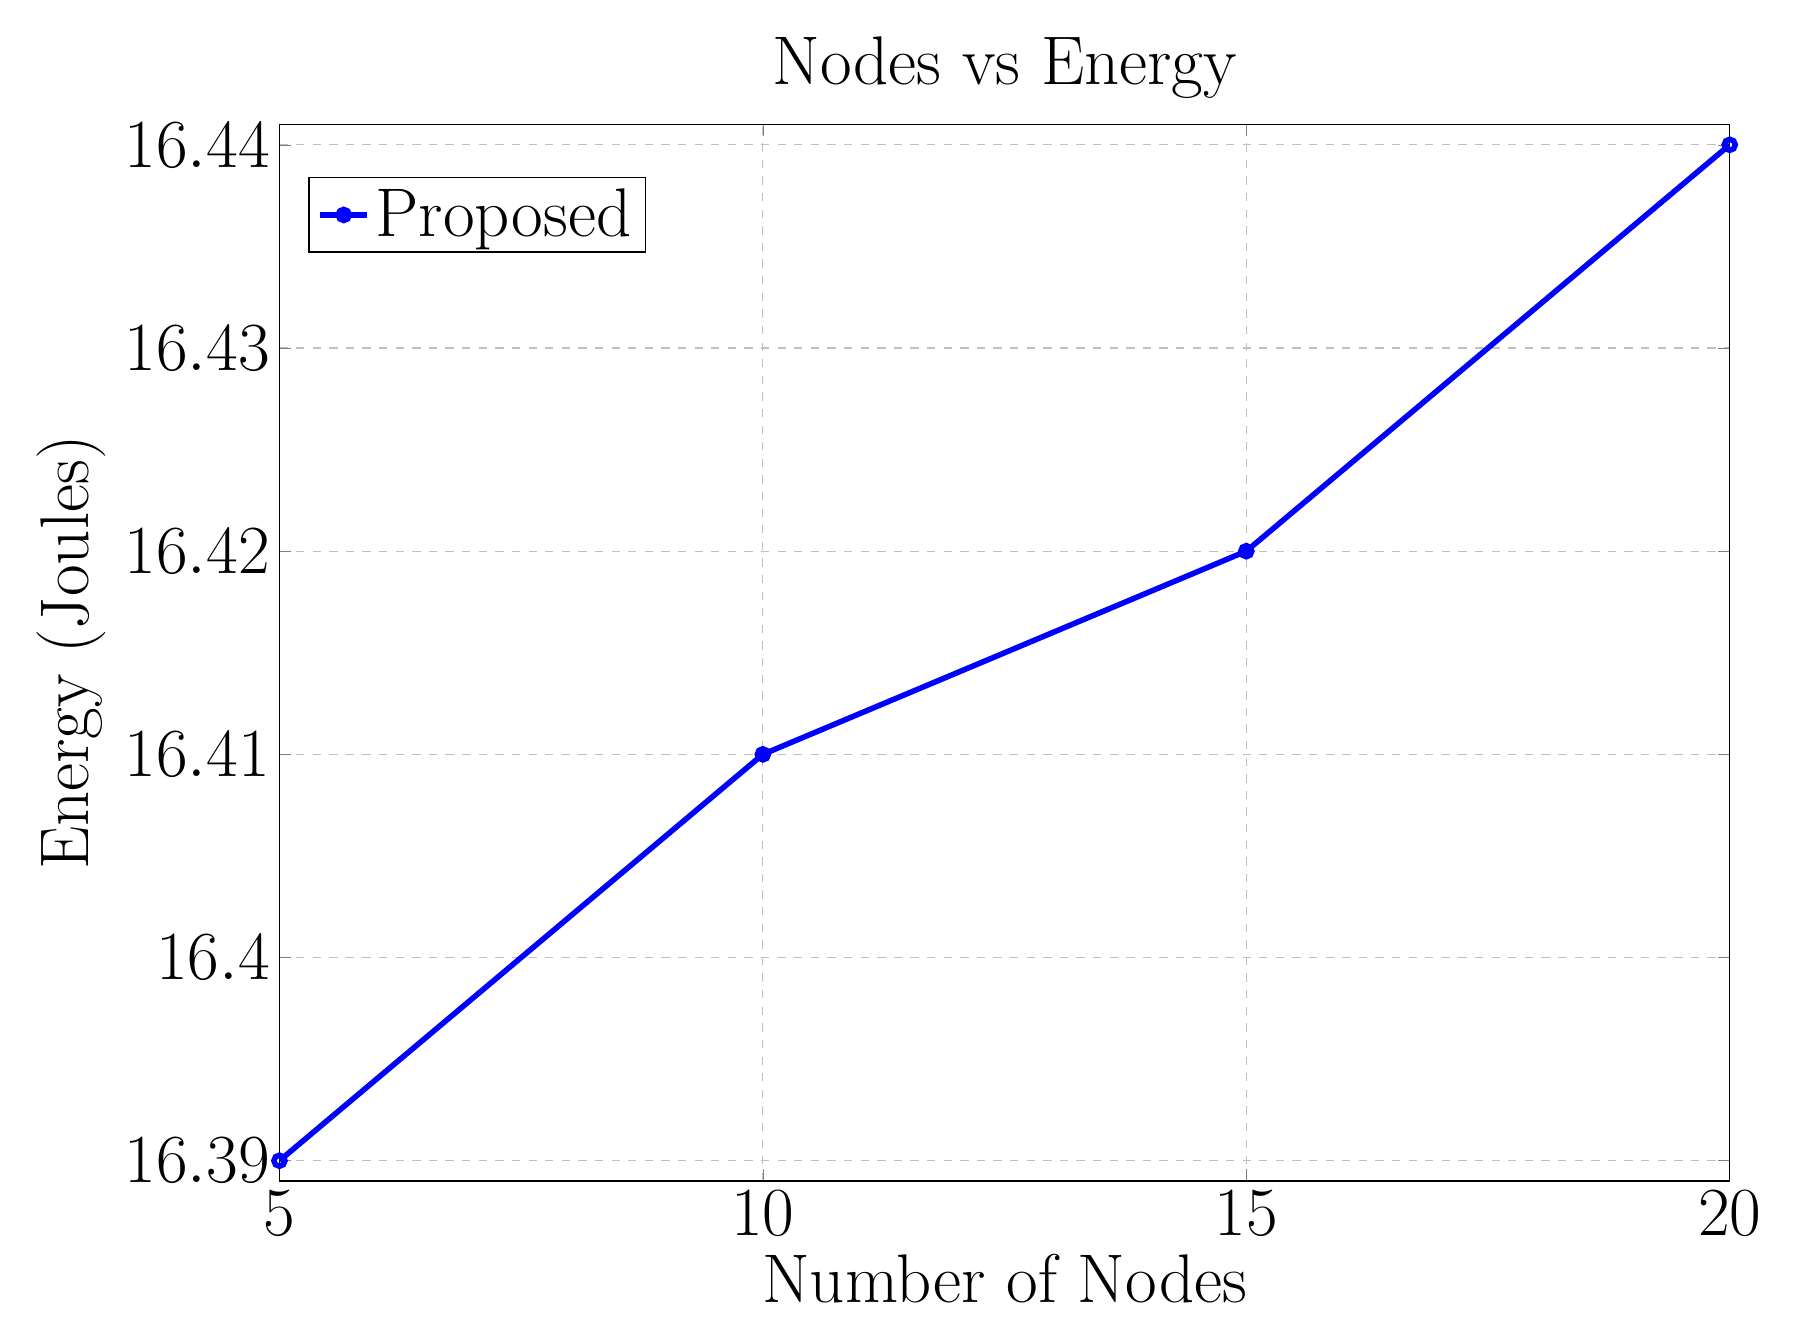
\begin{tikzpicture}
\begin{axis}[
 width=20cm,
 height=15cm,
 tick label style={font=\fontsize{24}{28}\selectfont},
 label style={font=\fontsize{24}{28}\selectfont},
 title style={font=\fontsize{24}{28}\selectfont},
 title={Nodes vs Energy},
 xlabel={Number of Nodes},
 ylabel={Energy (Joules)},
 xmin=5, xmax=20,
 ymin=16.389, ymax=16.441,
 xtick={5,10,15,20},
 ytick={16.39,16.40,16.41,16.42,16.43,16.44},
 legend style={
 font=\fontsize{24}{28}\selectfont,
 at={(0.02,0.95)},
 anchor=north west,
 draw=black,
 fill=white
 },
 ymajorgrids=true,
 xmajorgrids=true,
 grid style=dashed
]

% Energy line
\addplot+[mark=o,color=blue,line width=2pt] coordinates {
 (5,16.39)(10,16.41)(15,16.42)(20,16.44)
};

\legend{Proposed}

\end{axis}
\end{tikzpicture}
\end{document}